\documentclass[9pt]{beamer}

% Beamer style
%\usetheme[secheader]{Madrid}
% \usetheme{CambridgeUS}
\useoutertheme{infolines}
\usecolortheme[rgb={0.65,0.15,0.25}]{structure}
% \usefonttheme[onlymath]{serif}
\beamertemplatenavigationsymbolsempty
%\AtBeginSubsection

% Packages
%\usepackage[french]{babel}
\usepackage[latin1]{inputenc}
\usepackage{color}
% \usepackage[dvipsnames]{xcolor}
\usepackage{xspace}
\usepackage{dsfont, stmaryrd}
\usepackage{amsmath, amsfonts, amssymb, stmaryrd, mathabx}
\usepackage{epsfig}
\usepackage{multirow}
\usepackage{tikz}
\usepackage{url}
% \usepackage{ulem}
\usepackage{/home/robin/LATEX/Biblio/astats}
%\usepackage[all]{xy}
\usepackage{graphicx}

% Maths
% \newtheorem{theorem}{Theorem}
% \newtheorem{definition}{Definition}
\newtheorem{proposition}{Proposition}
% \newtheorem{assumption}{Assumption}
% \newtheorem{algorithm}{Algorithm}
% \newtheorem{lemma}{Lemma}
% \newtheorem{remark}{Remark}
% \newtheorem{exercise}{Exercise}
% \newcommand{\propname}{Prop.}
% \newcommand{\proof}{\noindent{\sl Proof:}\quad}
% \newcommand{\eproof}{$\blacksquare$}

% \setcounter{secnumdepth}{3}
% \setcounter{tocdepth}{3}
\newcommand{\pref}[1]{\ref{#1} p.\pageref{#1}}
\newcommand{\qref}[1]{\eqref{#1} p.\pageref{#1}}

% Colors : http://latexcolor.com/
\definecolor{darkred}{rgb}{0.65,0.15,0.25}
\definecolor{darkgreen}{rgb}{0,0.4,0}
\definecolor{darkred}{rgb}{0.65,0.15,0.25}
\definecolor{amethyst}{rgb}{0.6, 0.4, 0.8}
\definecolor{asparagus}{rgb}{0.53, 0.66, 0.42}
\definecolor{applegreen}{rgb}{0.55, 0.71, 0.0}
\definecolor{awesome}{rgb}{1.0, 0.13, 0.32}
\definecolor{blue-green}{rgb}{0.0, 0.87, 0.87}
\definecolor{red-ggplot}{rgb}{0.52, 0.25, 0.23}
\definecolor{green-ggplot}{rgb}{0.42, 0.58, 0.00}
\definecolor{purple-ggplot}{rgb}{0.34, 0.21, 0.44}
\definecolor{blue-ggplot}{rgb}{0.00, 0.49, 0.51}

% Commands
\newcommand{\backupbegin}{
   \newcounter{finalframe}
   \setcounter{finalframe}{\value{framenumber}}
}
\newcommand{\backupend}{
   \setcounter{framenumber}{\value{finalframe}}
}
\newcommand{\emphase}[1]{\textcolor{darkred}{#1}}
\newcommand{\comment}[1]{\textcolor{gray}{#1}}
\newcommand{\paragraph}[1]{\textcolor{darkred}{#1}}
\newcommand{\refer}[1]{{\small{\textcolor{gray}{{\cite{#1}}}}}}
\newcommand{\Refer}[1]{{\small{\textcolor{gray}{{[#1]}}}}}
\newcommand{\goto}[1]{{\small{\textcolor{blue}{[\#\ref{#1}]}}}}
\renewcommand{\newblock}{}

\newcommand{\tabequation}[1]{{\medskip \centerline{#1} \medskip}}
% \renewcommand{\binom}[2]{{\left(\begin{array}{c} #1 \\ #2 \end{array}\right)}}

% Variables 
\newcommand{\Abf}{{\bf A}}
\newcommand{\Beta}{\text{B}}
\newcommand{\Bcal}{\mathcal{B}}
\newcommand{\Bias}{\xspace\mathbb B}
\newcommand{\Cor}{{\mathbb C}\text{or}}
\newcommand{\Cov}{{\mathbb C}\text{ov}}
\newcommand{\cl}{\text{\it c}\ell}
\newcommand{\Ccal}{\mathcal{C}}
\newcommand{\cst}{\text{cst}}
\newcommand{\Dcal}{\mathcal{D}}
\newcommand{\Ecal}{\mathcal{E}}
\newcommand{\Esp}{\xspace\mathbb E}
\newcommand{\Espt}{\widetilde{\Esp}}
\newcommand{\Covt}{\widetilde{\Cov}}
\newcommand{\Ibb}{\mathbb I}
\newcommand{\Fcal}{\mathcal{F}}
\newcommand{\Gcal}{\mathcal{G}}
\newcommand{\Gam}{\mathcal{G}\text{am}}
\newcommand{\Hcal}{\mathcal{H}}
\newcommand{\Jcal}{\mathcal{J}}
\newcommand{\Lcal}{\mathcal{L}}
\newcommand{\Mt}{\widetilde{M}}
\newcommand{\mt}{\widetilde{m}}
\newcommand{\Nbb}{\mathbb{N}}
\newcommand{\Mcal}{\mathcal{M}}
\newcommand{\Ncal}{\mathcal{N}}
\newcommand{\Ocal}{\mathcal{O}}
\newcommand{\pt}{\widetilde{p}}
\newcommand{\Pt}{\widetilde{P}}
\newcommand{\Pbb}{\mathbb{P}}
\newcommand{\Pcal}{\mathcal{P}}
\newcommand{\Qcal}{\mathcal{Q}}
\newcommand{\qt}{\widetilde{q}}
\newcommand{\Rbb}{\mathbb{R}}
\newcommand{\Sbb}{\mathbb{S}}
\newcommand{\Scal}{\mathcal{S}}
\newcommand{\st}{\widetilde{s}}
\newcommand{\St}{\widetilde{S}}
\newcommand{\Tcal}{\mathcal{T}}
\newcommand{\todo}{\textcolor{red}{TO DO}}
\newcommand{\Ucal}{\mathcal{U}}
\newcommand{\Un}{\math{1}}
\newcommand{\Vcal}{\mathcal{V}}
\newcommand{\Var}{\mathbb V}
\newcommand{\Vart}{\widetilde{\Var}}
\newcommand{\Zcal}{\mathcal{Z}}

% Symboles & notations
\newcommand\independent{\protect\mathpalette{\protect\independenT}{\perp}}\def\independenT#1#2{\mathrel{\rlap{$#1#2$}\mkern2mu{#1#2}}} 
\renewcommand{\d}{\text{\xspace d}}
\newcommand{\gv}{\mid}
\newcommand{\ggv}{\, \| \, }
% \newcommand{\diag}{\text{diag}}
\newcommand{\card}[1]{\text{card}\left(#1\right)}
\newcommand{\trace}[1]{\text{tr}\left(#1\right)}
\newcommand{\matr}[1]{\boldsymbol{#1}}
\newcommand{\matrbf}[1]{\mathbf{#1}}
\newcommand{\vect}[1]{\matr{#1}} %% un peu inutile
\newcommand{\vectbf}[1]{\matrbf{#1}} %% un peu inutile
\newcommand{\trans}{\intercal}
\newcommand{\transpose}[1]{\matr{#1}^\trans}
\newcommand{\crossprod}[2]{\transpose{#1} \matr{#2}}
\newcommand{\tcrossprod}[2]{\matr{#1} \transpose{#2}}
\newcommand{\matprod}[2]{\matr{#1} \matr{#2}}
\DeclareMathOperator*{\argmin}{arg\,min}
\DeclareMathOperator*{\argmax}{arg\,max}
\DeclareMathOperator{\sign}{sign}
\DeclareMathOperator{\tr}{tr}
\newcommand{\ra}{\emphase{$\rightarrow$} \xspace}

% Hadamard, Kronecker and vec operators
\DeclareMathOperator{\Diag}{Diag} % matrix diagonal
\DeclareMathOperator{\diag}{diag} % vector diagonal
\DeclareMathOperator{\mtov}{vec} % matrix to vector
\newcommand{\kro}{\otimes} % Kronecker product
\newcommand{\had}{\odot}   % Hadamard product

% TikZ
\newcommand{\nodesize}{2em}
\newcommand{\edgeunit}{2.5*\nodesize}
\newcommand{\edgewidth}{1pt}
\tikzstyle{node}=[draw, circle, fill=black, minimum width=.75\nodesize, inner sep=0]
\tikzstyle{square}=[rectangle, draw]
\tikzstyle{param}=[draw, rectangle, fill=gray!50, minimum width=\nodesize, minimum height=\nodesize, inner sep=0]
\tikzstyle{hidden}=[draw, circle, fill=gray!50, minimum width=\nodesize, inner sep=0]
\tikzstyle{hiddenred}=[draw, circle, color=red, fill=gray!50, minimum width=\nodesize, inner sep=0]
\tikzstyle{observed}=[draw, circle, minimum width=\nodesize, inner sep=0]
\tikzstyle{observedred}=[draw, circle, minimum width=\nodesize, color=red, inner sep=0]
\tikzstyle{eliminated}=[draw, circle, minimum width=\nodesize, color=gray!50, inner sep=0]
\tikzstyle{empty}=[draw, circle, minimum width=\nodesize, color=white, inner sep=0]
\tikzstyle{blank}=[color=white]
\tikzstyle{nocircle}=[minimum width=\nodesize, inner sep=0]

\tikzstyle{edge}=[-, line width=\edgewidth]
\tikzstyle{edgebendleft}=[-, >=latex, line width=\edgewidth, bend left]
\tikzstyle{edgebendright}=[-, >=latex, line width=\edgewidth, bend right]
\tikzstyle{lightedge}=[-, line width=\edgewidth, color=gray!50]
\tikzstyle{lightedgebendleft}=[-, >=latex, line width=\edgewidth, bend left, color=gray!50]
\tikzstyle{lightedgebendright}=[-, >=latex, line width=\edgewidth, bend right, color=gray!50]
\tikzstyle{edgered}=[-, line width=\edgewidth, color=red]
\tikzstyle{edgebendleftred}=[-, >=latex, line width=\edgewidth, bend left, color=red]
\tikzstyle{edgebendrightred}=[-, >=latex, line width=\edgewidth, bend right, color=red]

\tikzstyle{arrow}=[->, >=latex, line width=\edgewidth]
\tikzstyle{arrowbendleft}=[->, >=latex, line width=\edgewidth, bend left]
\tikzstyle{arrowbendright}=[->, >=latex, line width=\edgewidth, bend right]
\tikzstyle{arrowred}=[->, >=latex, line width=\edgewidth, color=red]
\tikzstyle{arrowbendleftred}=[->, >=latex, line width=\edgewidth, bend left, color=red]
\tikzstyle{arrowbendrightred}=[->, >=latex, line width=\edgewidth, bend right, color=red]
\tikzstyle{arrowblue}=[->, >=latex, line width=\edgewidth, color=blue]
\tikzstyle{dashedarrow}=[->, >=latex, dashed, line width=\edgewidth]
\tikzstyle{dashededge}=[-, >=latex, dashed, line width=\edgewidth]
\tikzstyle{dashededgebendleft}=[-, >=latex, dashed, line width=\edgewidth, bend left]
\tikzstyle{lightarrow}=[->, >=latex, line width=\edgewidth, color=gray!50]

\newcommand{\dN}{\Delta N}
\newcommand{\dtau}{\Delta \tau}

% Directory
\newcommand{\figcp}{/home/robin/RECHERCHE/RUPTURES/EXPOSES/FIGURES}
% \newcommand{\figDLR}{/home/robin/Bureau/Hawkes/segHP/article/StatComp2023/Revision/figures}
\newcommand{\figchiro}{/home/robin/RECHERCHE/RUPTURES/Hawkes/HawkesDiscreteHMM/Figures/chiropteres}
\newcommand{\figsimul}{/home/robin/RECHERCHE/RUPTURES/Hawkes/HawkesDiscreteHMM/Figures/simuls}

%====================================================================
%====================================================================

%====================================================================
%====================================================================
\begin{document}
%====================================================================
%====================================================================

%====================================================================
\title{Markov-switching (discrete-time) Hawkes process}

\author[S. Robin]{S. Robin \\ \medskip
\begin{tabular}{rl}
  joint work with A. Bonnet 
\end{tabular}
% , E. Lebarbier, C. Dion-Blanc \refer{DLR24}
}

\institute[Sorbonne universit�]{\normalsize{LPSM, Sorbonne universit�}}

\date[Lancaster'25]{STOR-i, Lancaster, Jun. 2025}

%====================================================================
%====================================================================
\maketitle

%====================================================================
%====================================================================
\section*{Introduction}
%====================================================================
\frame{\frametitle{'Motivation'} 

  \begin{tabular}{cc}
    \hspace{-.04\textwidth}
    \begin{tabular}{p{.5\textwidth}}
      \paragraph{Counting process} \\
      Overnight recording of bat cries in continuous time
      
      \bigskip
      \begin{itemize}
        \setlength{\itemsep}{.75\baselineskip}
        \onslide+<3->{\item Can we detect changes in the occurrence of events?}
        \onslide+<4->{\item Can we associate each time period with some underlying behavior?}
      \end{itemize}
      \bigskip \bigskip 
    \end{tabular}
    & 
    \hspace{-.05\textwidth}
    \begin{tabular}{p{.5\textwidth}}
      \begin{overprint}
        \onslide<1>
        ~ \bigskip 
        \includegraphics[width=.45\textwidth]{\figcp/ChauveSouris-GrandBourg}
        \onslide<2>
        \includegraphics[width=.45\textwidth, trim=0 0 0 50, clip=]{\figchiro/Chiro-seq625-N1535-Qmax5-raw.png}
        \onslide<3>
        \includegraphics[width=.45\textwidth, trim=0 0 0 50, clip=]{\figchiro/Chiro-seq625-N1535-Qmax5-seg.png}
        \onslide<4->
        \includegraphics[width=.45\textwidth, trim=0 0 0 50, clip=]{\figchiro/Chiro-seq625-N1535-Qmax5-viterbi.png}
      \end{overprint}
    \end{tabular}
  \end{tabular}

  \onslide+<5>{\paragraph{Modelling.} Markov switching point process.}
}

%====================================================================
\frame{\frametitle{Point process} 

  \paragraph{Reminder.}
%   \vspace{-.1\textheight}
  $$
  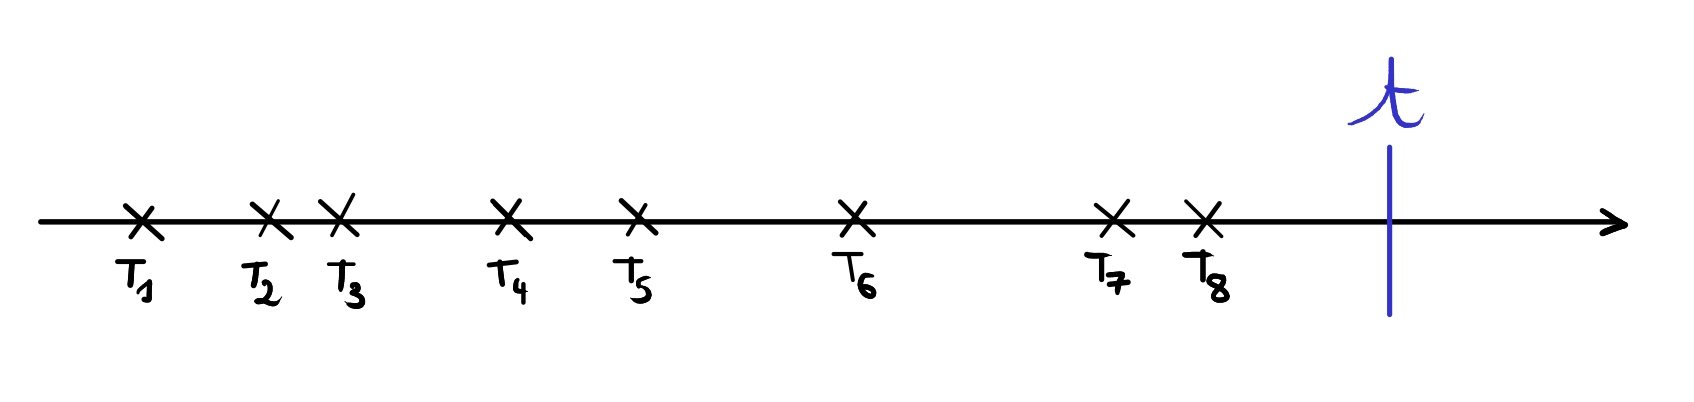
\includegraphics[width=.6\textwidth, trim=0 10 0 0, clip=]{\figcp/Bon24-Hawkes-Fig1}
  $$ 
  \begin{itemize}
    \setlength{\itemsep}{0.5\baselineskip}
    \item $(T_k)_{k \geq 1}$ a random collection of points
    \item Count process $H(t) = \sum_{k \geq 1} \Ibb\{T_k \leq t\}$
    \item Intensity function $\lambda(t)$: immediate probability of observing an event at time $t$
  \end{itemize}

  \bigskip \bigskip \pause
  \paragraph{Examples}
  \begin{itemize}
    \setlength{\itemsep}{0.5\baselineskip}
    \item{Homogeneous Poisson process:} $\lambda(t) \equiv \lambda$
    \item{Heterogeneous Poisson process:} $\lambda(t) =$ deterministic function
    \item{Hawkes process:} $\lambda(t) =$ random function of the past
  \end{itemize}
  
}

%====================================================================
%====================================================================
\section{(Discrete) Hawkes process}
\frame{\frametitle{Outline} \tableofcontents[currentsection]}
%====================================================================
\frame{\frametitle{Univariate Hawkes process} 

  $$
  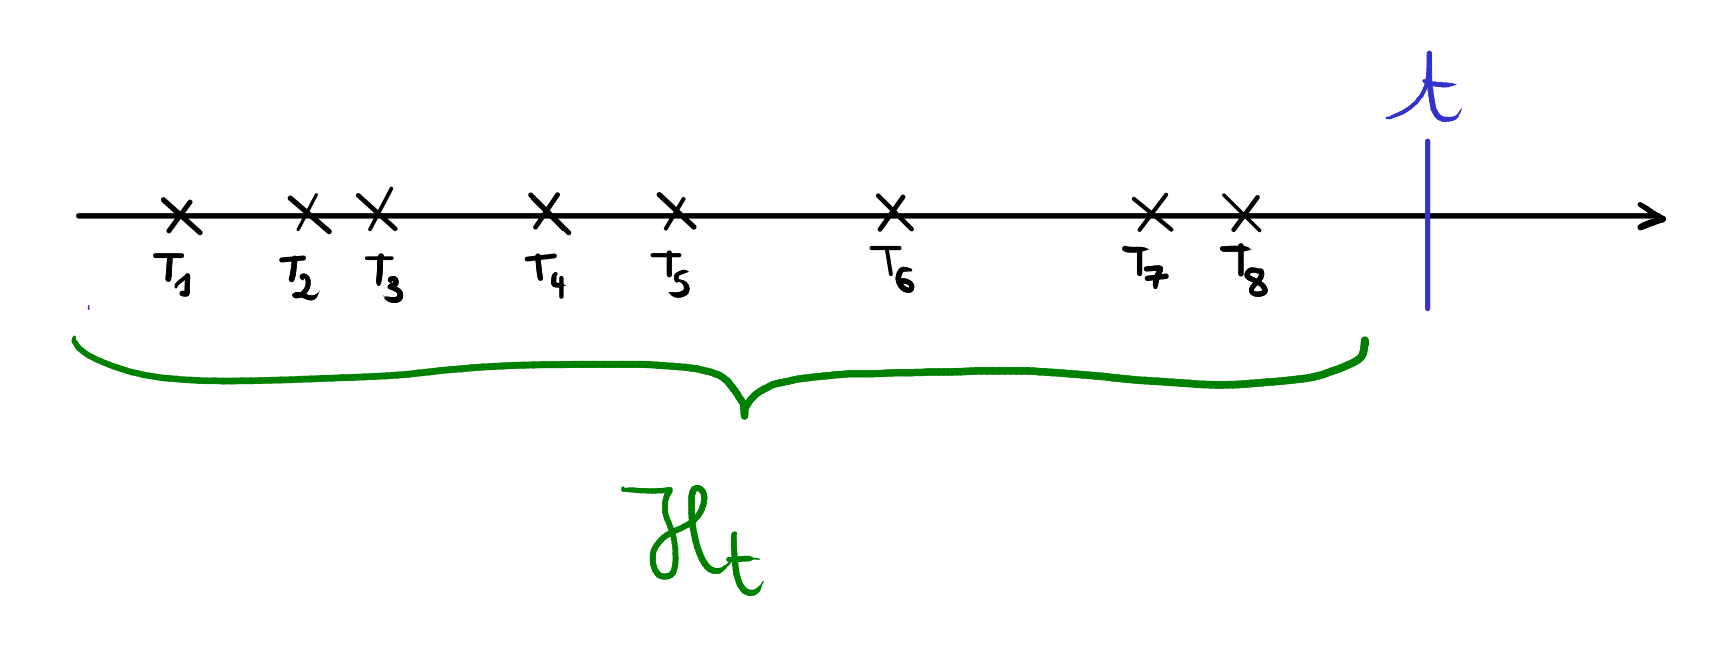
\includegraphics[width=.6\textwidth]{\figcp/Bon24-Hawkes-Fig2}
  $$
 
  \bigskip
  \paragraph{(Conditional) intensity function for the Hawkes process \refer{Haw71a}:}
  $$
  \lambda(t \mid \Hcal_t)= \lambda(t) = \lambda_0 + \underset{T_k < t}{\sum} h(t-T_k)
  $$
 %\nocite{Haw71b}
 
  \begin{itemize}
  \item $\lambda_0 =$ baseline 
  \item $h =$ kernel = influence of past events
  \end{itemize}

}

%====================================================================
\frame{\frametitle{Self-exciting exponential Hawkes process} 

  $$
  \lambda(t)= \lambda_0 + \underset{T_k < t}{\sum} a e^{-b(t-T_k)}
  $$
  \paragraph{Self exciting:} 
  Each event increases the probability of observing another event
  
  \bigskip \bigskip \pause
  \begin{tabular}{cc}
    \hspace{-.04\textwidth}
    \begin{tabular}{p{.4\textwidth}}
      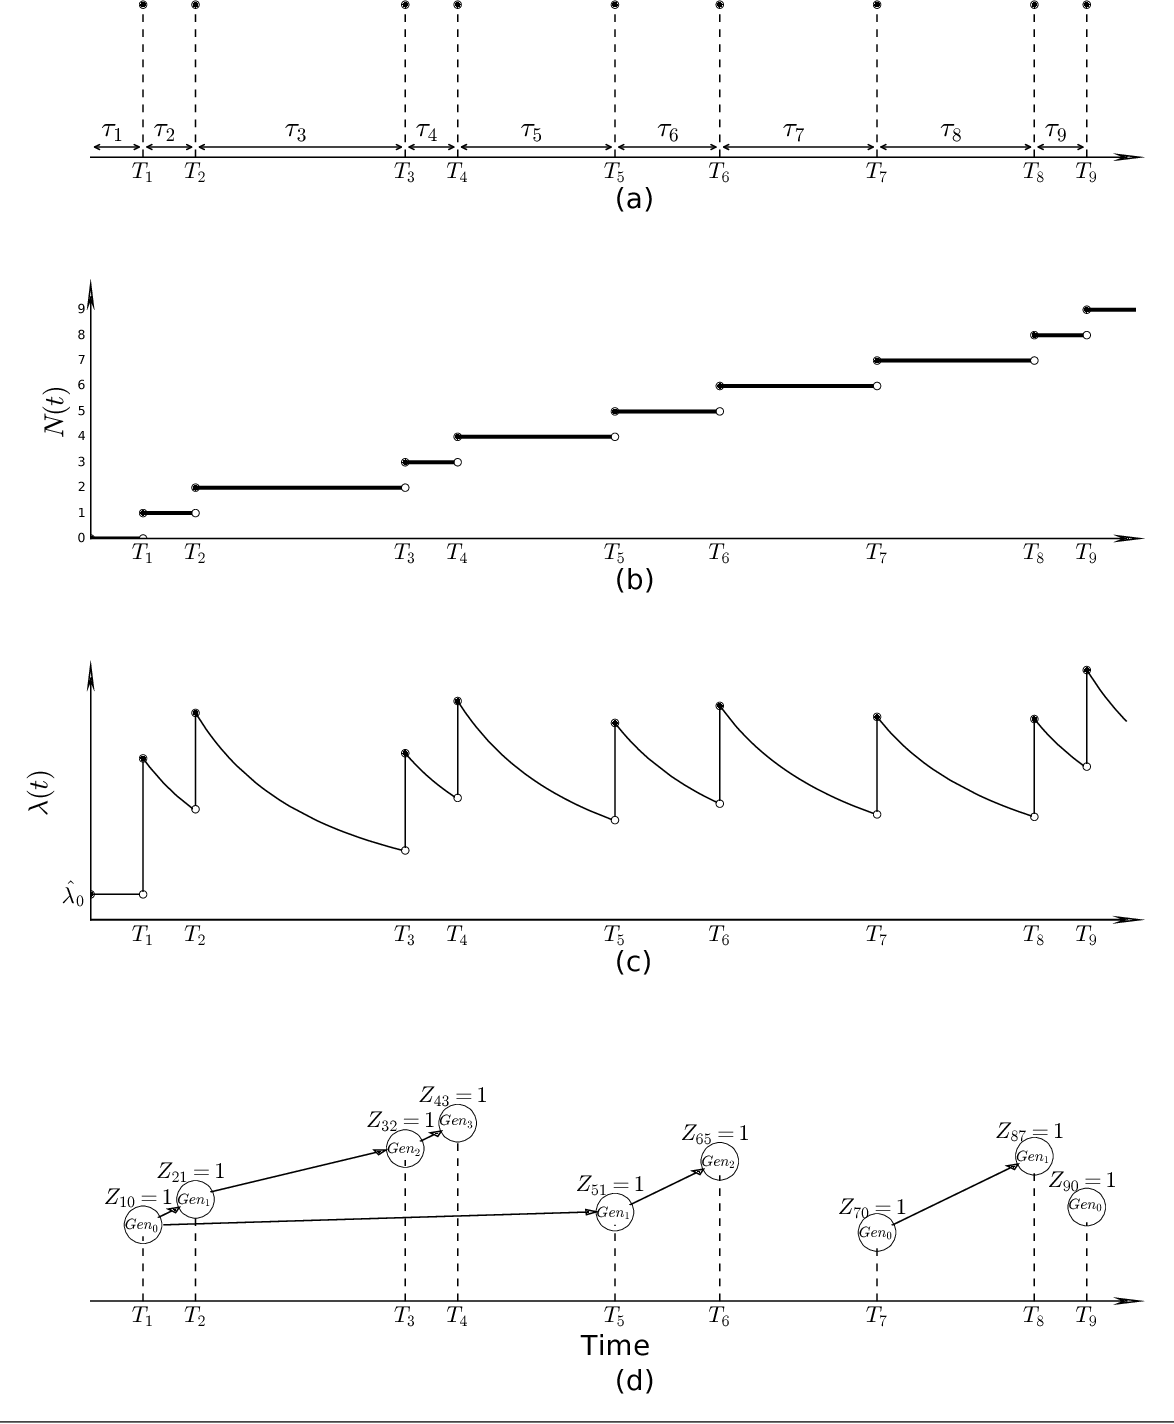
\includegraphics[width=.4\textwidth, trim=0 450 0 0, clip=]{\figcp/Bon24-Hawkes-Fig3}
    \end{tabular}
    & 
    \hspace{-.05\textwidth}
    \begin{tabular}{p{.55\textwidth}}
      \begin{itemize}
        \setlength{\itemsep}{1.5\baselineskip}
        \item Exponential kernel function \emphase{$h(t)= a e^{-b t}$}
        \item \emphase{$a \geq 0$} to ensure that $\lambda$ is non negative 
        \item \emphase{$a/b <1$} to ensure stationarity
        \item Applications: sismology, epidemiology, neuroscience, ecology, ...
      \end{itemize}
    \end{tabular}
  \end{tabular}  

}

%====================================================================
\frame{\frametitle{Cluster representation \refer{HaO74}} 

  $$
  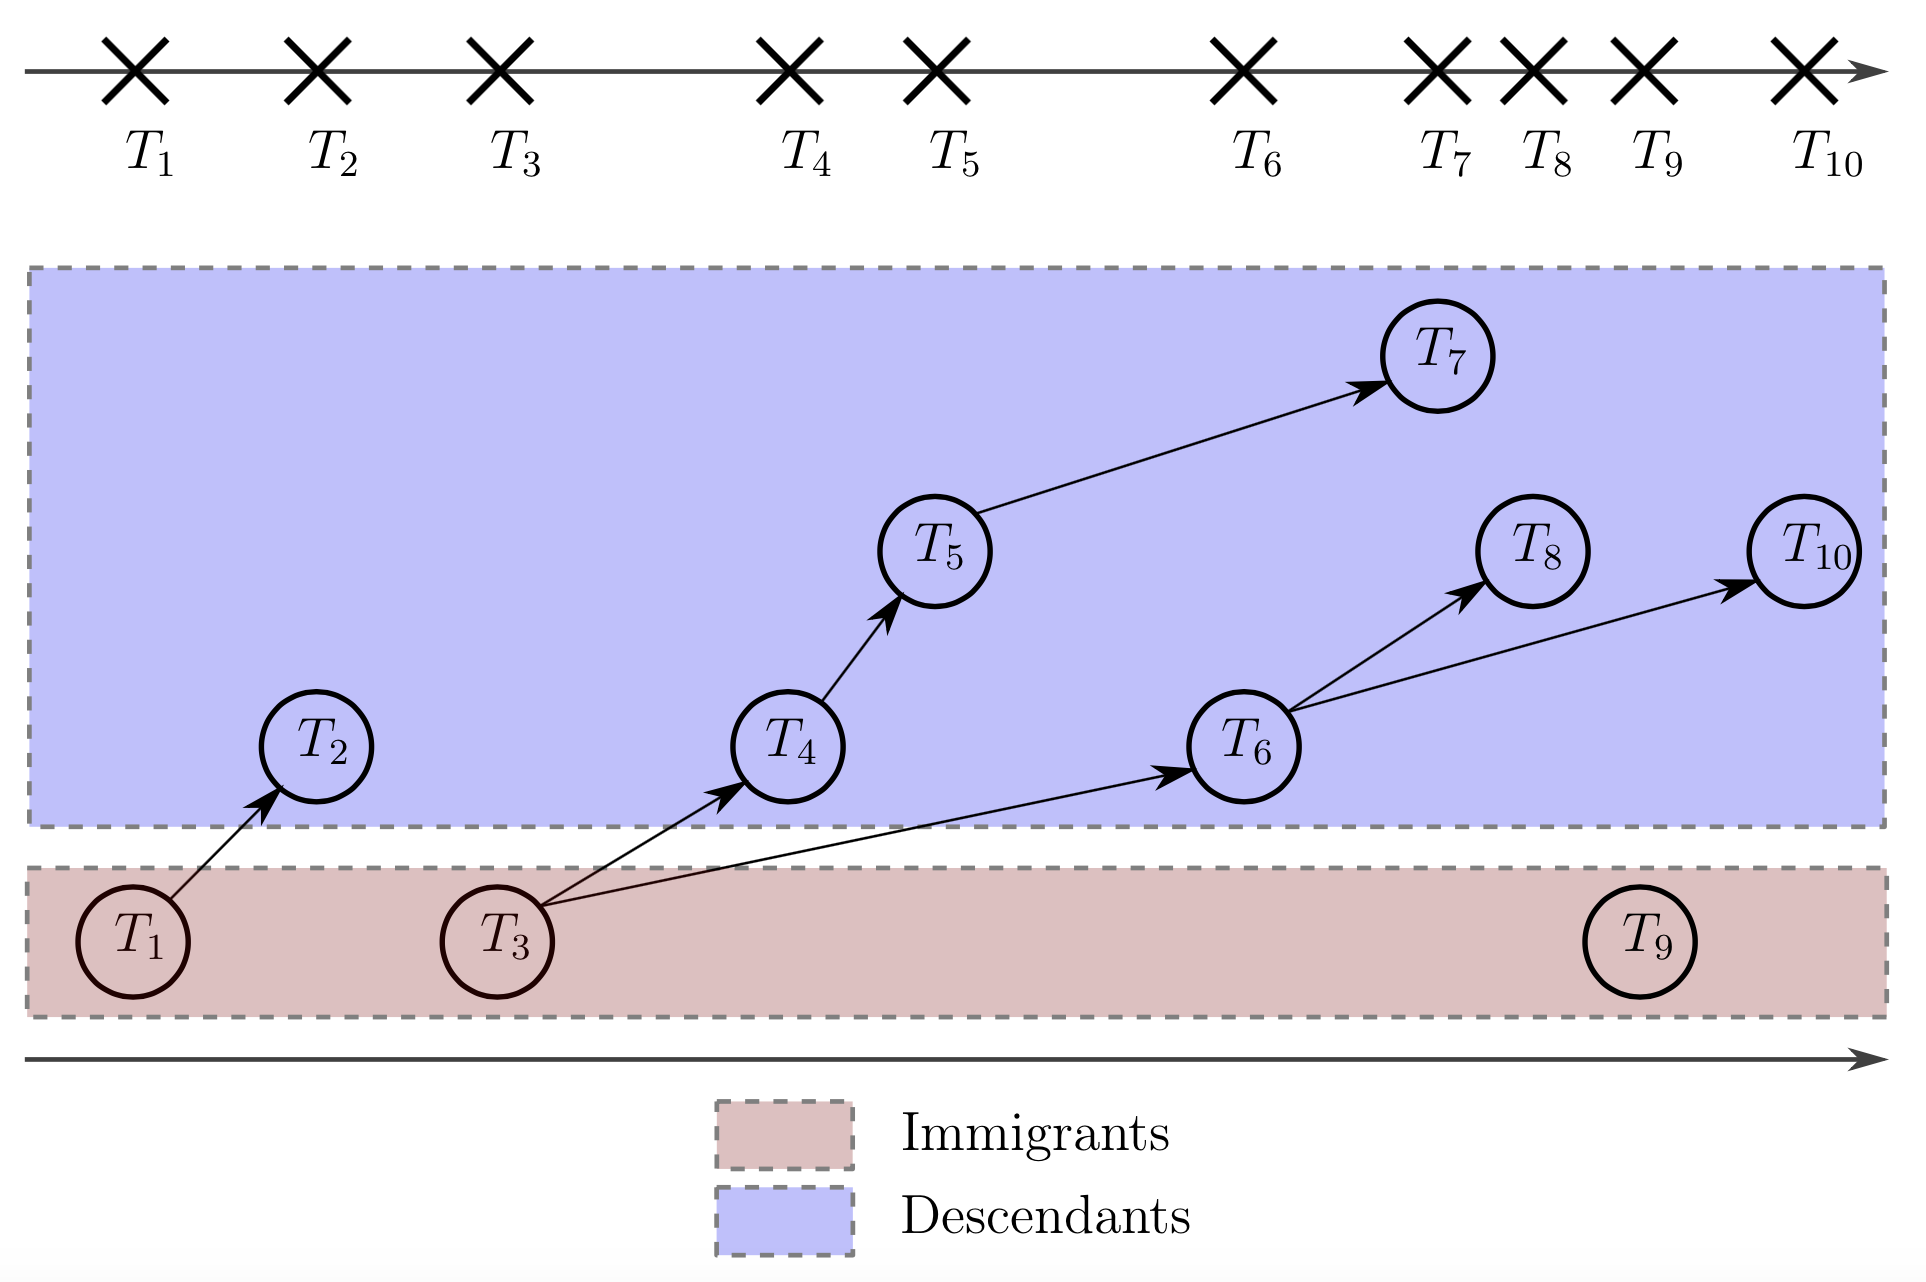
\includegraphics[width=.7\textwidth, trim=0 100 0 0 0, clip=]{\figcp/Bon24-Hawkes-Cluster}
  $$
  $$
  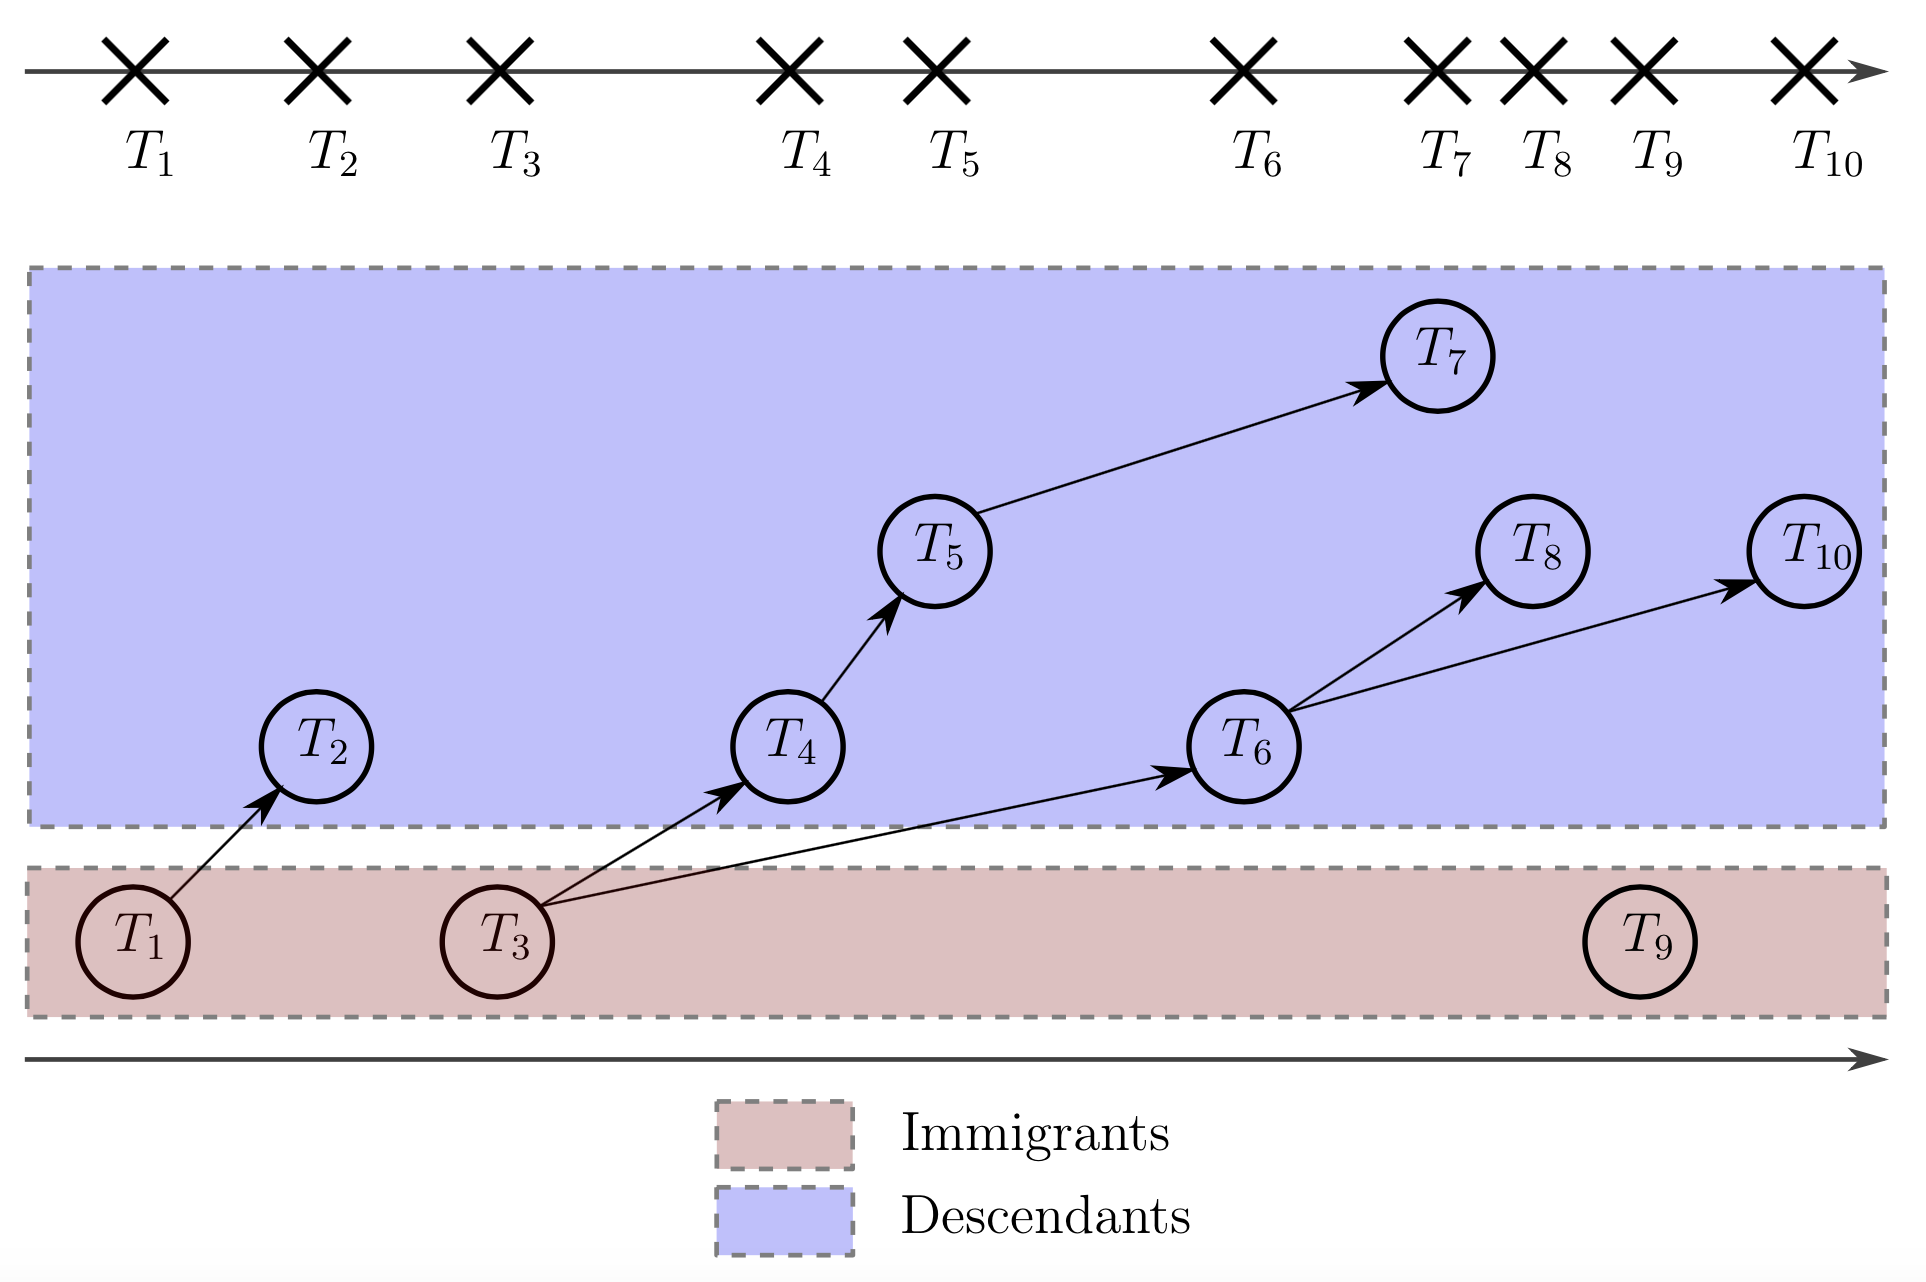
\includegraphics[width=.2\textwidth, trim=350 50 350 550, clip=]{\figcp/Bon24-Hawkes-Cluster}
  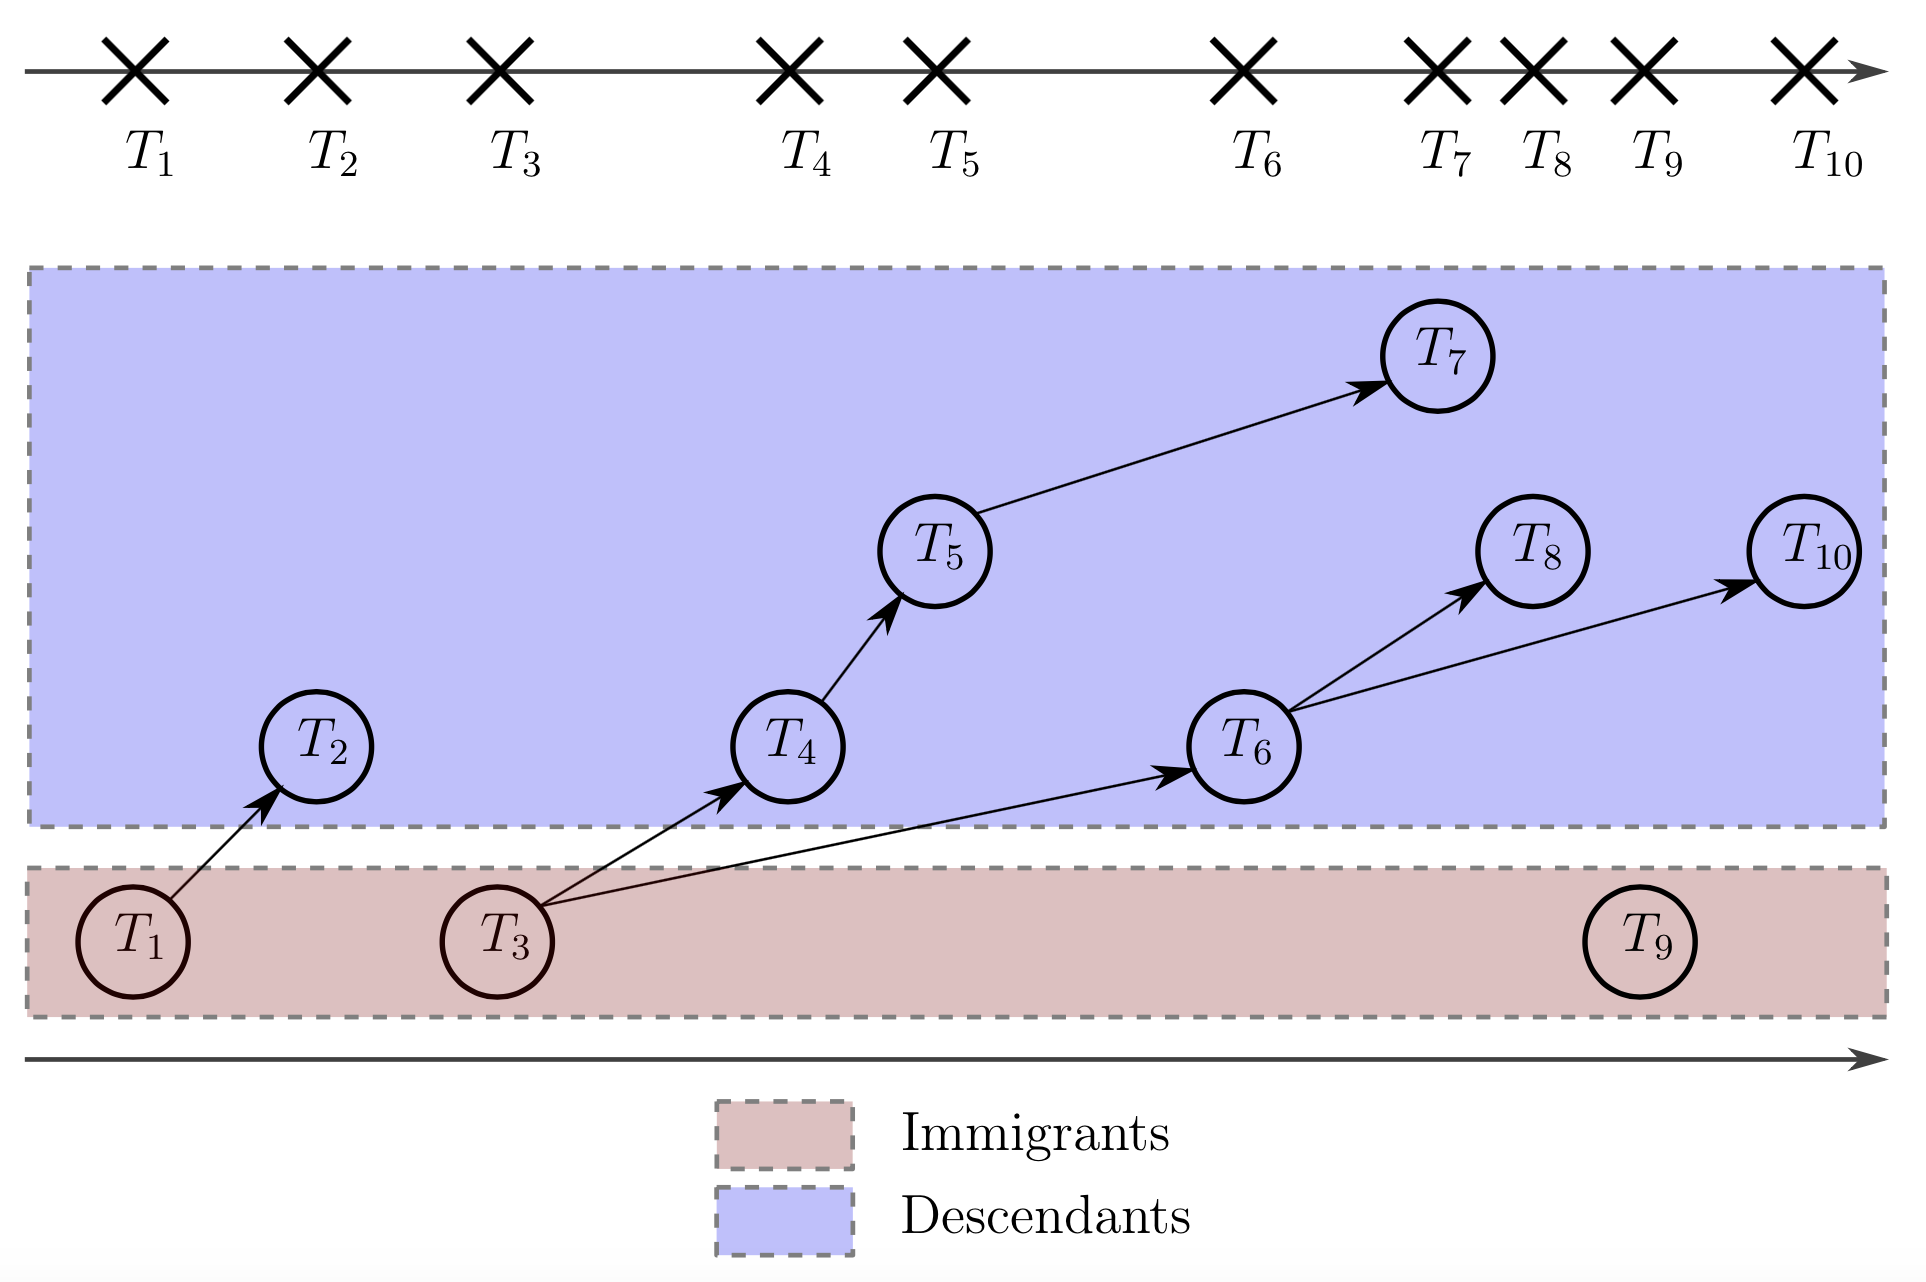
\includegraphics[width=.2\textwidth, trim=350 10 350 590, clip=]{\figcp/Bon24-Hawkes-Cluster}
  $$
%   \refer{HaO74}
  \begin{itemize}
  \item Immigrants arrive at rate $\lambda_0$ 
  \item Each immigrant or descendant produces new individuals at rate $h(t - T)$
  \end{itemize}

}

%====================================================================
\frame{\frametitle{Discrete time Hawkes process} 

\paragraph{Continuous time exponential Hawkes process}
$$
\lambda(t)=\lambda_0 + \underset{T_k < t}{\sum} a e^{-b(t-T_k)} 
$$    

\bigskip \bigskip \pause
\paragraph{Discretization} \refer{Seo15,Kir16,Kir17}
\begin{itemize}
  \setlength{\itemsep}{0.75\baselineskip}
  \item $I_k=[ \tau_{k-1};\tau_k]$ with $\tau_k=k\Delta$
  \item $H_k = H(I_k)$ the number of events on $I_k$
  $$
  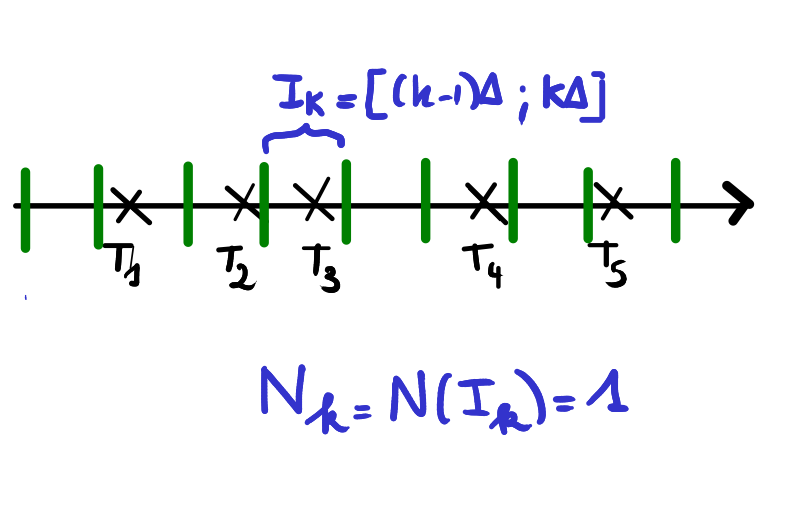
\includegraphics[width=.45\textwidth, trim=0 230 0 70, clip=]{\figcp/Bon24-Hawkes-Fig4}
  $$
  \item Distribution of $(H_k)_{k \geq 1}$?
\end{itemize}

}

%====================================================================
\frame{\frametitle{Discrete time Hawkes process} 

  $H_k$ number of events on $I_k=[ \tau_{k-1};\tau_k]$
  
  \bigskip \bigskip \pause
  \paragraph{Count distribution}
  $$
  H_k \overset{\Delta}{=} B_k + \sum_{\ell \leq k-1} \sum_{T \in I_\ell} M_T(I_k) + R_k
  $$
  \begin{itemize}
    \item $B_k \sim \mathcal{P}(\lambda_0 \Delta)$ discrete immigrant process
    \item $ M_T(I_k) \sim \mathcal{P}\left(c(a,b,\Delta) e^{-b(\tau_{k-1}-\emphase{T})}\right)$ descendants of $T<\tau_{k-1}$
    \item $R_k$ number of descendants of points $T \in I_k$ within $I_k$
  \end{itemize}

  \bigskip \bigskip \pause
  \paragraph{Approximation when $\Delta$ is small}
  \begin{itemize}
    \item  $ M_T(I_k) \simeq \mathcal{P}\left(c(a,b,\Delta) e^{-b(\tau_{k-1}-\emphase{\tau_{\ell-1}})}\right)$ for $T \in  I_\ell=[\tau_{\ell-1}; \tau_\ell]$
    \item \emphase{$R_k \simeq 0$}
  \end{itemize}
}

%====================================================================
\frame{\frametitle{Markovian reformulation} 

  \paragraph{Approximation of $H_k$}
  $$
  Y_k \mid (Y_\ell)_{\ell \leq k-1} \sim \mathcal{P}\left(\mu + \sum_{\ell = 1}^{k-1}\alpha \beta^{\ell-1} Y_{k-\ell} \right),
  $$
  with $\mu=\lambda_0 \Delta$ and $\alpha$, $\beta$ depending on $a$, $b$, $\Delta$.
  
  \bigskip
  \emphase{$\to$ $(Y_k)_{k\geq 1}$ is not a Markov chain} (infinite memory).

  \bigskip \bigskip \pause
  \paragraph{Markovian representation.}
  \begin{itemize}
    \item \pause Define
    \begin{align*}
      U_1 = 0, \qquad \qquad 
      U_k = \sum_{\ell = 1}^k \alpha \beta^{\ell-1} Y_{k-\ell}, 
    \end{align*} 
    \item \pause we have for $k \geq 1$ \textcolor{gray}{(with $U_0 = Y_0 = 0$)}
    \begin{align*}
      U_k = {\alpha Y_{k-1} + \beta U_{k-1}}, 
      \qquad \qquad 
      Y_k \mid U_k \sim \mathcal{P}(\mu + U_k).
    \end{align*}
  \end{itemize}
  \pause 
  \medskip
  \emphase{$\to$ $\left((Y_k,U_k)\right)_{k \geq 1}$ forms a Markov Chain}.
}

%====================================================================
\frame{\frametitle{Graphical model} 

  \paragraph{Discrete time Hawkes process.}
  $$
  (Y_k)_{k \geq 1} \sim Discrete~Hawkes(\mu, \alpha, \beta)
  $$
  \begin{align*}
    U_1 & = 0, &
    U_k & = \alpha Y_{k-1} + \beta U_{k-1}, & 
    Y_k & \sim \mathcal{P}(\mu + U_k)
  \end{align*}
  
  \bigskip \bigskip \pause
  \paragraph{Graphical model:}
  \begin{figure}
    \begin{centering}
    \begin{tikzpicture}
\node[] (Ut_1) at (-0.5*\edgeunit, 0.5*\edgeunit) {$U_{k-1}$}; 
\node[] (Ut) at (0.5*\edgeunit, 0.5*\edgeunit) {$U_{k}$}; 
\node[] (Ut1) at (1.5*\edgeunit, 0.5*\edgeunit) {$U_{k+1}$}; 
\node[] (Ut2) at (2.5*\edgeunit, 0.5*\edgeunit) {$U_{k+2}$}; 
\node[] (Ut3) at (3.5*\edgeunit, 0.5*\edgeunit) {}; 
\node[] (Yt_2) at (-\edgeunit, 0) {}; 
\node[] (Yt_1) at (0, 0) {$Y_{k-1}$}; 
\node[] (Yt) at (\edgeunit, 0) {$Y_{k}$}; 
\node[] (Yt1) at (2*\edgeunit, 0) {$Y_{k+1}$}; 
\node[] (Yt2) at (3*\edgeunit, 0) {}; 

\draw[->] (Ut_1) -- (Yt_1); \draw[->] (Ut) -- (Yt); \draw[->] (Ut1) -- (Yt1);
\draw[->] (Ut_1) -- (Ut); \draw[->] (Ut) -- (Ut1); \draw[->] (Ut1) -- (Ut2); \draw[->,dashed] (Ut2) -- (Ut3);
\draw[->,dashed] (Yt_2) -- (Ut_1); \draw[->] (Yt_1) -- (Ut); \draw[->] (Yt) -- (Ut1); \draw[->] (Yt1) -- (Ut2);
\end{tikzpicture}
 \\
    $\quad (U_k)_{k \geq 1} =$ \emphase{memory}, 
    $\quad (Y_k)_{k \geq 1} =$ \emphase{observed process}.
    \end{centering}
  \end{figure}
  
  \begin{align*}
    p\left(U_k, Y_k \mid (U_s, Y_s)_{s \leq k-1}\right)
    & =
    p\left(U_k, Y_k \mid U_{k-1}, Y_{k-1}\right) \\
    & =
    p\left(U_k \mid U_{k-1}, Y_{k-1}\right) p\left(Y_k \mid U_k\right)
  \end{align*}

}

%====================================================================
%====================================================================
\section{Discrete Markov switching Hawkes process}
\frame{\frametitle{Outline} \tableofcontents[currentsection]}
%====================================================================
\frame{\frametitle{Discrete time Hawkes HMM} 

  \paragraph{Model:} $Q$ hidden states
  \begin{itemize}
    \setlength{\itemsep}{.75\baselineskip}
    \item Hidden path: $(Z_k)_{k \geq 1}$ homogeneous Markov chain with transition matrix $\pi$
    \item \pause Observed counts: for $k\geq 1$ and
      $$
      Y_k \mid (Y_\ell)_{\ell \leq k-1} 
      \sim \mathcal{P}\left(\emphase{\mu_{Z_k}} + \sum_{\ell = 1}^{k-1} \alpha \beta^{\ell-1}Y_{k-\ell} \right)
      $$  
      or, for $k \geq 1$ \textcolor{gray}{(with $U_0 = Y_0 = 0$)}
      \begin{align*}
        U_k & = \alpha Y_{k-1} + \beta U_{k-1}, &
        Y_k & \mid U_k 
        \sim \mathcal{P}\left(\emphase{\mu_{Z_k}} + U_k \right)
      \end{align*}
  \end{itemize}
  
  \bigskip \bigskip \pause
  \paragraph{Assumptions:}
  \begin{itemize}
    \setlength{\itemsep}{1\baselineskip}
    \item The immigration rate $\mu$ varies with the hidden state
    \item The distribution of the number of offspring ($\alpha, \beta$) does not vary with the hidden state
  \end{itemize}

}

%====================================================================
\frame{\frametitle{Discrete time Hawkes HMM} 

  \paragraph{Graphical model:}
  \begin{figure}
    \begin{centering}
    \begin{tikzpicture}
\node[] (Zt_2) at (-\edgeunit, \edgeunit) {}; 
\node[] (Zt_1) at (0, \edgeunit) {$Z_{k-1}$}; 
\node[] (Zt) at (\edgeunit, \edgeunit) {$Z_{k}$}; 
\node[] (Zt1) at (2*\edgeunit, \edgeunit) {$Z_{k+1}$}; 
\node[] (Zt2) at (3*\edgeunit, \edgeunit) {}; 
\node[] (Ut_1) at (-0.5*\edgeunit, 0.5*\edgeunit) {$U_{k-1}$}; 
\node[] (Ut) at (0.5*\edgeunit, 0.5*\edgeunit) {$U_{k}$}; 
\node[] (Ut1) at (1.5*\edgeunit, 0.5*\edgeunit) {$U_{k+1}$}; 
\node[] (Ut2) at (2.5*\edgeunit, 0.5*\edgeunit) {$U_{k+2}$}; 
\node[] (Ut3) at (3.5*\edgeunit, 0.5*\edgeunit) {}; 
\node[] (Yt_2) at (-\edgeunit, 0) {}; 
\node[] (Yt_1) at (0, 0) {$Y_{k-1}$}; 
\node[] (Yt) at (\edgeunit, 0) {$Y_{k}$}; 
\node[] (Yt1) at (2*\edgeunit, 0) {$Y_{k+1}$}; 
\node[] (Yt2) at (3*\edgeunit, 0) {}; 

\draw[->,dashed] (Zt_2) -- (Zt_1); \draw[->] (Zt_1) -- (Zt); \draw[->] (Zt) -- (Zt1); \draw[->,dashed] (Zt1) -- (Zt2);
\draw[->] (Zt_1) -- (Yt_1); \draw[->] (Zt) -- (Yt); \draw[->] (Zt1) -- (Yt1);
\draw[->] (Ut_1) -- (Yt_1); \draw[->] (Ut) -- (Yt); \draw[->] (Ut1) -- (Yt1);
\draw[->] (Ut_1) -- (Ut); \draw[->] (Ut) -- (Ut1); \draw[->] (Ut1) -- (Ut2); \draw[->,dashed] (Ut2) -- (Ut3);
\draw[->,dashed] (Yt_2) -- (Ut_1); \draw[->] (Yt_1) -- (Ut); \draw[->] (Yt) -- (Ut1); \draw[->] (Yt1) -- (Ut2);
\end{tikzpicture}
 \\
    $(Z_k)_{k \geq 1} =$ \emphase{hidden path}, 
    $\quad (U_k)_{k \geq 1} =$ memory, 
    $\quad (Y_k)_{k \geq 1} =$ observed process.
    \end{centering}
  \end{figure}

  \bigskip \bigskip \pause
  \paragraph{Remarks:}
  \begin{itemize}
    \setlength{\itemsep}{.75\baselineskip}
    \item The memory of the past is 'stored' in the variable $U_k$, which can still be computed recursively ($U_k = \alpha Y_{k-1} + \beta U_{k-1}$)
    \item The Markovian property still holds if the influence of the past varies with the hidden state ($\alpha \to \alpha_k, \beta \to \beta_k$).
  \end{itemize}

}

%====================================================================
\frame{\frametitle{Identifiability}

  \paragraph{Proposition:} The model parameter $\theta = (\nu, \pi, (\mu_q)_{1 \leq q \leq Q}, \alpha, \beta)$ is identifiable from the joint distribution $p_\theta(Y_1, Y_2, Y_3)$:
  $$
  \theta' \neq \theta \qquad \Rightarrow \qquad p_{\theta'}^{Y_1, Y_2, Y_3} \neq p_\theta^{Y_1, Y_2, Y_3}.
  $$
  
  \bigskip \pause
  \paragraph{Sketch of proof.}Finite Poisson mixtures are identifiable \refer{Tei61}, so, because\footnote{The generic technique from \refer{AMR09} does not apply here.} 
  $$
%   {\Pr}_\theta\{Y_1=x, Y_2=y, Y_3=z\} 
  p_\theta^{Y_1, Y_2, Y_3}(x, y, z) 
  = \sum_{1 \leq q, \ell, m \leq Q} \nu_q \pi_{q\ell} \pi_{\ell m} \Pcal(x; \mu_q) \Pcal(y; \mu_\ell + \alpha x)  \Pcal(z; \mu_m + \alpha \beta x + \alpha y),
  $$
  \begin{enumerate}
    \setlength{\itemsep}{.75\baselineskip}
    \item \pause $\nu$ and $\mu$ can be identified from $p_\theta(Y_1)$, 
    \item \pause then $\alpha$ can be identified from $p_\theta(Y_2 \mid Y_1=1)$, 
    \item \pause then $\beta$ can be identified from $p_\theta(Y_3 \mid Y_1=1, Y_2=0)$, 
    \item \pause then $\pi$ can be identified from the joint mixture
    $$
%     {\Pr}_\theta\{Y_1=x, Y_2=y\} 
    p_\theta^{Y_1, Y_2}(x, y) 
    = \sum_{1 \leq q, \ell \leq Q} \nu_q \pi_{q\ell} \Pcal(x; \mu_q) \Pcal(y; \mu_\ell + \alpha x),
    $$
    which is proven identifiable.
  \end{enumerate}

}

%====================================================================
\frame{\frametitle{Inference}

  \paragraph{Aim:} Infer the parameter $\theta$
  $$
  \widehat{\theta} = \argmax_\theta \log p_\theta(Y)
  $$

  \bigskip \bigskip \pause
  \paragraph{EM algorithm for HMM:} \refer{DLR77,CMR05}
  $$
  \theta^{(h+1)} 
  = \underset{\text{\normalsize \emphase{M step}}}{\underbrace{\argmax_\theta}} \; \underset{\text{\normalsize \emphase{E step}}}{\underbrace{\Esp_{\theta^{(h)}}}}[\log p_\theta(Y, Z) \mid Y]
  $$
  \begin{itemize}
    \setlength{\itemsep}{.75\baselineskip}
    \item E step: Evaluate $Q(\theta \mid \theta^{(h)}) = \Esp_{\theta^{(h)}}[\log p_\theta(Y, Z) \mid Y]$ (forward-backward recursion)
    \item M step: Gradient descent, computing $\nabla_\theta Q(\theta \mid \theta^{(h)})$ by recursion
  \end{itemize}

}

%====================================================================
\frame{\frametitle{Inference}

  \paragraph{Classification:} 
  \begin{align*}
    \text{Marginal:} & & 
    \widehat{Z}_k & = \argmax_q P_{\widehat{\theta}}\{Z_k = q \mid Y \}, \\
    \text{Joint (Viterbi):} & & 
    \widehat{Z} & = \argmax_z P_{\widehat{\theta}}\{Z=z \mid Y\} 
  \end{align*}

  \bigskip \bigskip \pause
  \paragraph{Model selection:} Penalized likelihood
  \begin{align*}
    AIC_Q & = \log p_{\widehat{\theta}_Q}(Y) - D_Q, \\
    BIC_Q & = \log p_{\widehat{\theta}_Q}(Y) - D_Q \frac{\log(\emphase{N})}2     
  \end{align*}
  with $D_Q =$ number of parameters $= 2 + Q^2$ and \emphase{$N =$ number of time bins}.
}

%====================================================================
%====================================================================
\section{Simulation study}
\frame{\frametitle{Outline} \tableofcontents[currentsection]}
%====================================================================
\frame{ \frametitle{Simulation design}
  % Version V8 / tol=1e-6

  \begin{itemize}
    \setlength{\itemsep}{1.5\baselineskip}
    \item \emphase{Baseline continuous parameters:} $a^0 = 40$, $b^0 = 160$, 
    $$
    Q = 1: m^0 = [400], \quad
    Q = 2: m^0 = [10, \;800], \quad
    Q = 3: m^0 = [10, \;200, \;1000]
    $$
    \item \pause \emphase{Increasing signal:}
    $$
    a = \lambda \; a^0, \qquad 
    m = \lambda \; m^0, \qquad 
    \lambda = 0.5, \;1, \;1.5, \;2.
    $$ 
    \item \pause \emphase{Simulated process:}
    $$
    (H_t)_{0 \leq t \leq 1} \sim Heterogeneous~\emphase{Continuous}~Hawkes(a, b^0, m)
    $$
    \item \pause \emphase{Discretized process:} $n = H(1)$
    $$
    N = c \; n, \qquad c = 0.5, \;1, \;2, \;4,
    $$
    $$
    Y_k = H\left(\left[\frac{k-1}{N}; \frac{k}{N}\right]\right), 
    \qquad k=1, \dots N.
    $$
  \end{itemize}

}

%====================================================================
\frame{ \frametitle{Simulation results ($Q^* = 3$)}

  \begin{overprint}
    \onslide<1> \paragraph{Parameter estimates.} Distribution of $\widehat{\theta} - \theta^*$ ($Q = Q^*$) \\
    \includegraphics[width=1\textwidth, height=.8\textheight]{\figsimul/SimHHMM1DV8-tol6-T1-Q3-Coef-discParmsV2}
    \onslide<2> \paragraph{Model selection: BIC.} Distribution of $BIC_Q - BIC_1$ \\
    \includegraphics[width=1\textwidth, height=.8\textheight]{\figsimul/SimHHMM1DV8-tol6-T1-Q3-Coef-BIC}
    \onslide<3> \paragraph{Model selection: AIC.} Distribution of $AIC_Q - AIC_1$ \\
    \includegraphics[width=1\textwidth, height=.8\textheight]{\figsimul/SimHHMM1DV8-tol6-T1-Q3-Coef-AIC}
%     \onslide<4> \paragraph{Comparison with Poisson HMM.} $AIC_{1, Q^*, \widehat{Q}}(Poisson)$ / $AIC_{1, Q^*, \widehat{Q}}(Hawkes)$ \\
%     \includegraphics[width=1\textwidth, height=.8\textheight]{\figsimul/SimHHMM1DV8-tol6-T1-Q3-Coef-compAIC}
  \end{overprint}
}
    
%====================================================================
\frame{ \frametitle{Simulation conclusions}

  \begin{itemize}
    \setlength{\itemsep}{1\baselineskip}
    \item Inference easier when more signal (large $\lambda$)!!!
    \item Inference easier with thinner discretization step (large $N$) \\
    But higher computational cost 
    \item BIC does not capture the right number of states \\
    \textcolor{gray}{Sequences not simulated according to the model}
    \item AIC does, with reasonable signal ($\lambda$) and discretization ($N$) \\
    \textcolor{gray}{Blind to the simulation shift from the model?}
%     \item Clear advantage wrt Poisson HMM.
  \end{itemize}
  
  \bigskip \bigskip \pause
  \paragraph{Practical recommendations.}
  $$
  \text{Take $N = 2 n$ and use AIC}
  $$
}
    
%====================================================================
%====================================================================
\section{Illustrations}
\frame{\frametitle{Outline} \tableofcontents[currentsection]}
%====================================================================
\frame{ \frametitle{Bat cries}

  \paragraph{Data set.} $1555$ overnight recordings all over France
  
%   \bigskip 
%   \begin{overprint}
%     \onslide<2> \paragraph{Model selection.} $n = $ nb events, $N = c \; n$, \quad top: $BIC$, bottom: $AIC$. 
%     $$
%     \includegraphics[width=1\textwidth, height=.6\textheight]{\figchiro/ResSeqData-Coef-Qhat}
%     $$
%   \end{overprint}
% }
% 
% %====================================================================
% \frame{ \frametitle{Illustrations}

  \bigskip \bigskip \pause
  \paragraph{Poisson vs Hawkes / Homogeneous vs HMM.} Best model based on AIC
  $$
%   \begin{tabular}{c|cccc}
%     Best & \multicolumn{2}{c}{Poisson} & \multicolumn{2}{c}{Hawkes} \\ 
%     model & Homo.  & HMM & Homo.  & HMM \\
%     \hline
%     Nb sequences & 34  & 24 & 353 & 1144 
%   \end{tabular}
  \begin{tabular}{r|cc|c}
    & Poisson & Hawkes & Total \\
    \hline
    Homogeneous & 34 & 353 & 387\\
    Hidden Markov  & 24 & \emphase{1144} & \emphase{1168} \\
    \hline
    Total & 58 & \emphase{1497} & 1555
  \end{tabular}
  $$
  \begin{itemize}
    \item Memory ($95\%$) and heterogeneity ($75\%$) are present in most sequences 
    \item Hawkes-HMM best fits almost 3 sequences out of 4.
  \end{itemize}
}

%====================================================================
\frame{ \frametitle{Example}

  $$
  \begin{tabular}{cc}
    Hawkes HMM ($\widehat{Q} = 3$) & 
    Poisson HMM ($\widehat{Q} = 4$) \\ 
    \includegraphics[width=0.35\textwidth, trim=10 40 20 50, clip=]{\figchiro/Chiro-seq1776-N1048-Qmax5-classif} &
    \includegraphics[width=0.35\textwidth, trim=10 40 20 50, clip=]{\figchiro/Chiro-seq1776-N1048-Qmax5-classifP} 
  \end{tabular}
  $$
  \begin{itemize}
    \item Poisson-HMM needs many state changes to account for self-excitation
    \item Hawkes-HMM state change do not correspond to slope changes
  \end{itemize}

%   \begin{overprint}
%     \onslide<1> \paragraph{A recording.}
%     $n = 1535, \; c = 1 : N = 1535, \quad \widehat{Q}= 3$ \\ ~
%     $$
%     \begin{tabular}{ccc}
%       marginal classification & Viterbi & Model selection \\
%       $\widehat{Z}_k$ & $\widehat{Z}$ & \textcolor{red}{Hawkes} / \textcolor{blue}{Poisson} \\ 
%       \includegraphics[width=.3\textwidth, height=.4\textheight]{\figchiro/Chiro-seq625-N1535-Qmax5-classif} &
%       \includegraphics[width=.3\textwidth, height=.4\textheight]{\figchiro/Chiro-seq625-N1535-Qmax5-viterbi} &
%       \includegraphics[width=.3\textwidth, height=.4\textheight]{\figchiro/Chiro-seq625-N1535-Qmax5-models} \\
%       & & -- $\log L$, - - $BIC$, $\cdots AIC$
%     \end{tabular}
%     $$
%     \onslide<2> \paragraph{Another recording.}
%     $n = 1391, \; c = 1 : N = 1391, \quad \widehat{Q}= 3$ \\ ~
%     $$
%     \begin{tabular}{ccc}
%       marginal classification & Viterbi & Model selection \\
%       $\widehat{Z}_k$ & $\widehat{Z}$ & \textcolor{red}{Hawkes} / \textcolor{blue}{Poisson} \\ 
%       \includegraphics[width=.3\textwidth, height=.4\textheight]{\figchiro/Chiro-seq1530-N1391-Qmax5-classif} &
%       \includegraphics[width=.3\textwidth, height=.4\textheight]{\figchiro/Chiro-seq1530-N1391-Qmax5-viterbi} &
%       \includegraphics[width=.3\textwidth, height=.4\textheight]{\figchiro/Chiro-seq1530-N1391-Qmax5-models} \\     
%       & & -- $\log L$, - - $BIC$, $\cdots AIC$
%     \end{tabular}
%     $$
%     \onslide<3> \paragraph{Another recording.}
%     $n = 1574, \; c = 4 : N = 6296, \quad \widehat{Q}= 3$ 
%     $$
%     \begin{tabular}{ccc}
%       marginal classification & Viterbi & Model selection \\
%       $\widehat{Z}_k$ & $\widehat{Z}$ & \textcolor{red}{Hawkes} / \textcolor{blue}{Poisson} \\ 
%       \includegraphics[width=.3\textwidth, height=.4\textheight]{\figchiro/Chiro-seq2283-N6296-Qmax5-classif} &
%       \includegraphics[width=.3\textwidth, height=.4\textheight]{\figchiro/Chiro-seq2283-N6296-Qmax5-viterbi} &
%       \includegraphics[width=.3\textwidth, height=.4\textheight]{\figchiro/Chiro-seq2283-N6296-Qmax5-models} \\
%       & & -- $\log L$, - - $BIC$, $\cdots AIC$
%     \end{tabular}
%     $$
%   \end{overprint}
}
    
%====================================================================
\frame{ \frametitle{States and species}

  The number of bat species was also recorded 
  
  $$
  \includegraphics[width=.45\textwidth]{\figchiro/boxplot_species_Coef2_allQ.pdf}
  $$
  \begin{itemize}
    \item The number of states does not match the number of species
  \end{itemize}

}

%====================================================================
%====================================================================
\section{Discussion}
\frame{\frametitle{Outline} \tableofcontents[currentsection]}
%====================================================================
\frame{ \frametitle{Summary}

  \paragraph{What we did.} \\ ~
  \begin{itemize}
    \setlength{\itemsep}{1.25\baselineskip}
    \item The discretized Hawkes process with exponential kernel is a Markov model \\
    ~ \\
    $\Rightarrow$ The discretized Markov switching Hawkes process with exponential kernel is a hidden Markov model
    \item The standard EM machinery applies to achieve maximum likelihood inference.
    \item Not shown: initialization based on existing estimation procedures for homogeneous Hawkes and Poisson HMM.
  \end{itemize}
}
    
%====================================================================
\frame{ \frametitle{Discussion}

  \paragraph{What we did not do.} \\ ~
  \begin{itemize}
    \setlength{\itemsep}{1.25\baselineskip}
    \item Goodness-of-fit: 'Poissonisation' (on-going). \\
%     \item Model selection: BIC does not seem to work: why? \\
%     (simulation scheme, wrong derivation of the BIC, ...?)
    \item Identifiability: Needs to be proven. \\
    (standard HMM-dedicated strategies does not apply here \refer{AMR09}).
    \item Understand the inferred latent states in terms of animal behavior \& biogeography. \\
    (transit vs hunting, different species, ...)
  \end{itemize}


  \bigskip \bigskip \pause
  \paragraph{In parallel.} With C. Dion-Blanc, E. Lebarbier et D. Hawat 
  \begin{itemize}
    \setlength{\itemsep}{0.75\baselineskip}
    \item Efficient change-point detection ('segmentation') in Poisson \& Hawkes processes \refer{DHL24}. \\
    (Dynamic programming applies.)
    \item Segmentation-classification of Poisson processes.
  \end{itemize}

}
    
%====================================================================
\frame{ \frametitle{References}
  {
   \footnotesize
   \bibliography{/home/robin/Biblio/BibGene}
   \bibliographystyle{alpha}
  }
}

%====================================================================
%====================================================================
\backupbegin 
\section*{Backup}
%====================================================================
\frame{ \frametitle{Discrete HMM}

  \paragraph{Conversion formulas} from continuous to discrete Hawkes
  $$
  \alpha  = \frac{e^{b \Delta} - 1}{b}, \qquad \beta = e^{-b \Delta}
  $$
    
  \bigskip \pause 
  \paragraph{3-step initialization}
  \begin{itemize}
    \setlength{\itemsep}{1\baselineskip}
    \item Homogeneous Hawkes for the reproduction parameters $\alpha$ and $\beta$ \\
    ({\tt hawkesbow} R package \refer{Che21})
    \item Poisson-HMM for the rates $\mu_1, \dots, \mu_Q$ and transition $\pi$
    \item Correction $\mu_k \rightarrow \widetilde{\mu}_k$ to account for reproduction rate
  \end{itemize}
  
}

% %====================================================================
% \frame{ \frametitle{Simulation results ($Q^* = 3$, fixed $N$)}
% 
%   \begin{overprint}
%     \onslide<1> \paragraph{Parameter estimates.} Distribution of $\widehat{\theta} - \theta^*$ ($Q = Q^*$) \\
%     \includegraphics[width=1\textwidth, height=.8\textheight]{\figsimul/SimHHMM1DV8-tol6-T1-Q3-N-discParmsV2}
%     \onslide<2> \paragraph{Model selection: BIC.} Distribution of $BIC_Q - BIC_1$ \\
%     \includegraphics[width=1\textwidth, height=.8\textheight]{\figsimul/SimHHMM1DV8-tol6-T1-Q3-N-BIC}
%     \onslide<3> \paragraph{Model selection: AIC.} Distribution of $AIC_Q - AIC_1$ \\
%     \includegraphics[width=1\textwidth, height=.8\textheight]{\figsimul/SimHHMM1DV8-tol6-T1-Q3-N-AIC}
%     \onslide<4> \paragraph{Comparison with Poisson HMM.} $AIC_{1, Q^*, \widehat{Q}}(Poisson)$ / $AIC_{1, Q^*, \widehat{Q}}(Hawkes)$ \\
%     \includegraphics[width=1\textwidth, height=.8\textheight]{\figsimul/SimHHMM1DV8-tol6-T1-Q3-N-compAIC}
%   \end{overprint}
% }
    
%====================================================================
\frame{ \frametitle{Simulation results ($Q^* = 1$, $N = c n$)}

  \begin{overprint}
    \onslide<1> \paragraph{Parameter estimates.} Distribution of $\widehat{\theta} - \theta^*$ ($Q = Q^*$) \\
    \includegraphics[width=1\textwidth, height=.8\textheight]{\figsimul/SimHHMM1DV8-tol6-T1-Q1-Coef-discParmsV2}
    \onslide<2> \paragraph{Model selection: BIC.} Distribution of $BIC_Q - BIC_1$ \\
    \includegraphics[width=1\textwidth, height=.8\textheight]{\figsimul/SimHHMM1DV8-tol6-T1-Q1-Coef-BIC}
    \onslide<3> \paragraph{Model selection: AIC.} Distribution of $AIC_Q - AIC_1$ \\
    \includegraphics[width=1\textwidth, height=.8\textheight]{\figsimul/SimHHMM1DV8-tol6-T1-Q1-Coef-AIC}
%     \onslide<4> \paragraph{Comparison with Poisson HMM.} $AIC_{1, Q^*, \widehat{Q}}(Poisson)$ / $AIC_{1, Q^*, \widehat{Q}}(Hawkes)$ \\
%     \includegraphics[width=1\textwidth, height=.8\textheight]{\figsimul/SimHHMM1DV8-tol6-T1-Q1-Coef-compAIC}
  \end{overprint}
}
    
%====================================================================
\frame{ \frametitle{Simulation results ($Q^* = 2$, $N = c n$)}

  \begin{overprint}
    \onslide<1> \paragraph{Parameter estimates.} Distribution of $\widehat{\theta} - \theta^*$ ($Q = Q^*$) \\
    \includegraphics[width=1\textwidth, height=.8\textheight]{\figsimul/SimHHMM1DV8-tol6-T1-Q2-Coef-discParmsV2}
    \onslide<2> \paragraph{Model selection: BIC.} Distribution of $BIC_Q - BIC_1$ \\
    \includegraphics[width=1\textwidth, height=.8\textheight]{\figsimul/SimHHMM1DV8-tol6-T1-Q2-Coef-BIC}
    \onslide<3> \paragraph{Model selection: AIC.} Distribution of $AIC_Q - AIC_1$ \\
    \includegraphics[width=1\textwidth, height=.8\textheight]{\figsimul/SimHHMM1DV8-tol6-T1-Q2-Coef-AIC}
%     \onslide<4> \paragraph{Comparison with Poisson HMM.} $AIC_{1, Q^*, \widehat{Q}}(Poisson)$ / $AIC_{1, Q^*, \widehat{Q}}(Hawkes)$ \\
%     \includegraphics[width=1\textwidth, height=.8\textheight]{\figsimul/SimHHMM1DV8-tol6-T1-Q2-Coef-compAIC}
  \end{overprint}
}
    
% %====================================================================
% \frame{ \frametitle{Backup: GoF}
% 
%   \paragraph{Change-time} for the recording of bat cries over one night:
%   $$
%   \begin{tabular}{cccc}
%     $Q = 1$ & $Q = 2$ & $Q = 3$ & $Q = 4$ \\
%     \includegraphics[width=.2\textwidth, height=.4\textheight, trim=20 20 20 20, clip=]{\figchiro/Chiro-seq99-N692-Qmax5-Q1gof} &
%     \includegraphics[width=.2\textwidth, height=.4\textheight, trim=20 20 20 20, clip=]{\figchiro/Chiro-seq99-N692-Qmax5-Q2gof} &
%     \includegraphics[width=.2\textwidth, height=.4\textheight, trim=20 20 20 20, clip=]{\figchiro/Chiro-seq99-N692-Qmax5-Q3gof} &
%     \includegraphics[width=.2\textwidth, height=.4\textheight, trim=20 20 20 20, clip=]{\figchiro/Chiro-seq99-N692-Qmax5-Q4gof}   
%     \end{tabular}
%   $$
% 
% }

%====================================================================
\frame{ \frametitle{States and locations}

  $$
  \begin{tabular}{cc}
    \includegraphics[width=0.4\textwidth]{\figchiro/Carte_Qmean.pdf} & \includegraphics[width=0.4\textwidth]{\figchiro/carte_species.pdf} \\
    \includegraphics[width=0.4\textwidth]{\figchiro/Carte_Qmean_bin.pdf} & \includegraphics[width=0.4\textwidth]{\figchiro/carte_species_bin.pdf} 
  \end{tabular}
  $$

}

%====================================================================
\backupend 

%====================================================================
%====================================================================
\end{document}
%====================================================================
%====================================================================
  
  \begin{tabular}{cc}
    \hspace{-.04\textwidth}
    \begin{tabular}{p{.5\textwidth}}
    \end{tabular}
    & 
    \hspace{-.02\textwidth}
    \begin{tabular}{p{.5\textwidth}}
    \end{tabular}
  \end{tabular}


